\section{Section Title}\label{sec:pageOne}

\subsection{Subection Title}\label{ssec:ssecOne}
\subsubsection{Subsubection Title}\label{sssec:sssecOne}
\paragraph{Paragraph Title}\label{par:parOne}~\\

This is an example of a \{table\} containing \textbackslash{}centering and a \{tabular\}, the table contains example of:
\begin{table}[H]
	\centering
	\captionof{table}{Table of Examples}
	\begin{tabular}{ | C{.45\textwidth} | C{.45\textwidth} | } \hline
		\textbf{TeX} & \textbf{Formatted} \\ \hline
		\textbackslash{}textbf\{Bold text\} & \textbf{Bold text} \\
		\textbackslash{}textit\{italicized text\} & \textit{italicized text} \\
		\{\textbackslash{}monof command\} & {\monof command} \\
		\textbackslash{}textbackslash & \textbackslash \\
		\textbackslash{}tildecentre & \textasciitilde \\
		1\textbackslash{}textsuperscript\{st\} & 1\textsuperscript{st} \\
		Philips\textbackslash{}textsubscript\{13\} & Philips\textsubscript{13} \\
		\textbackslash{}label\{[label]\} & [Invisible label of [name]] \\
		\textbackslash{}autoref\{[sectionOneLabel]\} & \autoref{sec:pageOne} \\
		\textbackslash{}textregistered & \textregistered \\
		\textbackslash{}textrightarrow & \textrightarrow \\
		\hline
	\end{tabular}
\end{table}

et cetera et cetera. Next is a \textbackslash{}\{figure\} which is \textbackslash{}caption-ed:

\begin{figure}[h!]
	\centering
	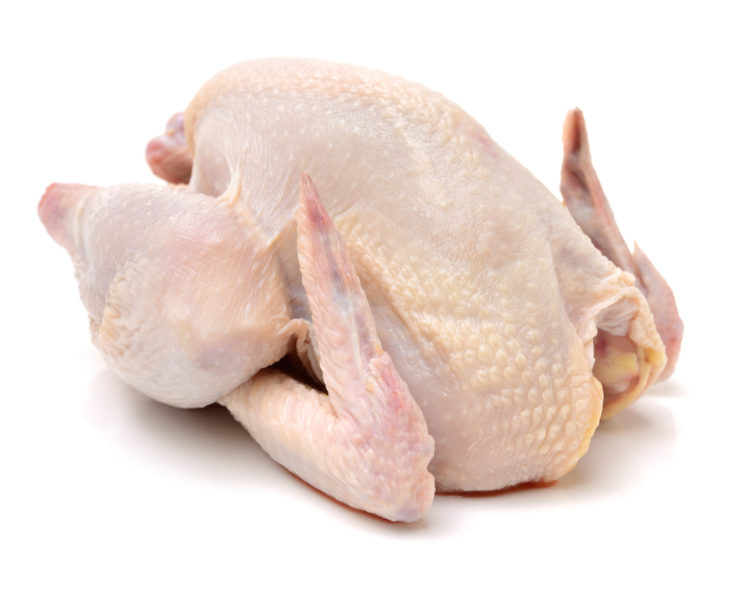
\includegraphics[scale=1]{exampleGRAPHIC.jpg}
	\caption{Example Figure/Graphic}
	\label{fig:example}
\end{figure}
